\chapter{Feasibility}
\label{ch:feasibility}

This chapter presents the preparation carried out so far and shows that the plan in
Chapter~\ref{ch:method} is achievable. Section~\ref{sec:env} describes the coding
environment, Section~\ref{sec:datasets} reviews the datasets, Section~\ref{sec:design}
presents the design, Section~\ref{sec:prototypes} reports the prototypes, and
Section~\ref{sec:feas-risks} summarises the main risks.

\section{Coding Environment}
\label{sec:env}

The system will be developed in Python. OpenCV \cite{bradski_opencv_2000} will be used for image
processing, PyTorch for the networks and Grad-CAM, and
matplotlib 
for the interface. Training will be ran on my own PC, and the code will be
kept under version control on GitHub. Python has been chosen as it has a wide range of libraries like PyTorch to help me speed up processing, and matplotlib is useful for graph reading.

\section{Datasets}
\label{sec:datasets}

\textbf{PTB-XL.} PTB-XL contains 21,800 ten-second twelve-lead ECGs, with diagnostic
labels and rhythm statements, and suggested patient-wise folds
\cite{wagner_ptbxl_2020}. Table~\ref{tab:class-counts} gives the number of records for each
class used in this project.

\begin{table}[ht]
  \centering
  \footnotesize
  \caption{Records per class in PTB-XL.}
  \label{tab:class-counts}
  \begin{tabular}{@{}p{0.45\linewidth} p{0.15\linewidth}@{}}
    \toprule
    \textbf{Class} & \textbf{Records} \\
    \midrule
    Normal & 9514 \\
    Myocardial infarction & 5469 \\
    ST/T change & 5235 \\
    Conduction disturbance & 4898 \\
    Hypertrophy & 2649 \\
    Atrial fibrillation & 1514 \\
    Atrial flutter & 73 \\
    Sinus tachycardia & 826 \\
    Sinus bradycardia & 637 \\
    \bottomrule
  \end{tabular}
\end{table}

There also might be Emory Healthcare to consider: However, I have not done the training for it yet (Mention to IDRIS)
\textbf{Real images.} The ECG-Image-Database provides 35,595 images of 1,977 recordings,
977 from PTB-XL and 1,000 from Emory Healthcare, printed, degraded and then scanned or
photographed \cite{reyna_ecg-image-database_2024}. The PTB-XL part can be matched to the
PTB-XL labels by record, which gives the labelled real test set; the Emory part uses
different labels.

\textbf{Limitations and preparation.} The classes are imbalanced, and the rare classes
have few cases, especially in the real-image subset, so some classes may only be evaluated
on rendered images. Labels come from at most two annotators \cite{wagner_ptbxl_2020} and
cardiologists can disagree \cite{dhutia_interrater_2017}. PTB-XL was collected in one period
with one manufacturer's devices, so models may not transfer to other settings. Preparation
consists of rendering images from the PTB-XL folds, converting labels to the nine classes,
and matching the real images to their labels.

% =====================================================================
\section{Design}
\label{sec:design}

Figure~\ref{fig:pipeline} shows the pipeline. An uploaded image is preprocessed, the trace
and beats are detected to give timing features, and the CNN uses the image and the timing
features to produce a probability for each class. Temperature scaling calibrates these
probabilities, and Grad-CAM produces a heatmap for each flagged class. The interface shows
the flags, the calibrated confidence, the heatmap and the measured values. The pipeline,
model and interface are separate modules, so any one can be replaced without changing the
others, for example swapping the pretrained model for the own CNN.

\begin{figure}[ht]
  \centering
  \fbox{\parbox{0.85\linewidth}{\centering Uploaded image $\rightarrow$
  preprocessing $\rightarrow$ trace and beat detection $\rightarrow$ timing features
  $+$ image $\rightarrow$ CNN $\rightarrow$ calibration $\rightarrow$ Grad-CAM
  $\rightarrow$ interface}}
  \caption{Planned system pipeline.}
  \label{fig:pipeline}
\end{figure}

The interface will have a student view, with the explanation and teaching support, and a clinician
view, with a short list of flags and measured values. Wireframe prototypes are listed in 

\begin{figure}[H]
  \centering
  \makebox[\linewidth][c]{%
  \begin{tikzpicture}[
      font=\small,
      mod/.style={draw, rounded corners=2pt, align=center, text width=28mm,
                  minimum height=11mm, fill=#1},
      mod/.default=blue!10,
      arr/.style={-{Latex[length=2mm]}, thick},
      lab/.style={font=\scriptsize, fill=white, inner sep=1pt}
    ]
    % analysis pipeline (middle column)
    \node[mod] (pre) at (0,0)      {Preprocessing\\\footnotesize OpenCV};
    \node[mod] (det) at (0,-19mm)  {Detection\\\footnotesize R peaks, HR, RR};
    \node[mod=orange!12] (clf) at (0,-38mm) {Classifier\\\footnotesize CNN (PyTorch)};
    \node[mod=orange!12] (cal) at (0,-57mm) {Calibration\\\footnotesize temperature $T$};
    \node[mod=orange!12] (exp) at (0,-76mm) {Explanation\\\footnotesize Grad-CAM};
    \node[draw, dashed, rounded corners, inner sep=3mm, fit=(pre)(exp),
          label={[font=\footnotesize\itshape]above:Analysis pipeline}] (pipe) {};

    % GUI (left)
    \node[mod=green!12, minimum height=86mm, text width=26mm, anchor=north]
         (gui) at (-56mm,5.5mm) {};
    \node[align=center, font=\small, text width=24mm, anchor=north] at (gui.north)
         {\textbf{GUI module}\\[3pt]Upload\\Results screen\\User view\\Clinical view};

    % offline training (right)
    \node[mod=black!5] (data) at (56mm,-10mm) {Data preparation\\\footnotesize ECG-Image-Kit, PTB-XL, ECG-Image-Database};
    \node[mod=black!5] (train) at (56mm,-36mm) {Training};
    \node[mod=black!5] (store) at (56mm,-62mm) {Saved model\\\footnotesize weights, $T$, thresholds};
    \node[draw, dashed, rounded corners, inner sep=3mm, fit=(data)(store),
          label={[font=\footnotesize\itshape]above:Offline training}] {};

    % pipeline flow
    \draw[arr] (pre) -- node[lab, right]{cleaned image, scale} (det);
    \draw[arr] (det) -- node[lab, right]{timing features} (clf);
    \draw[arr] (clf) -- node[lab, right]{class scores} (cal);
    \draw[arr] (cal) -- node[lab, right]{flagged classes} (exp);

    % GUI <-> pipeline
    \draw[arr] (gui.east |- 0,2.5mm) -- node[lab, above]{image} ([yshift=2.5mm]pre.west);
    \draw[arr] ([yshift=-2.5mm]pre.west) -- node[lab, below]{quality warning} (gui.east |- 0,-2.5mm);
    \draw[arr] (det.west) -- node[lab, above]{HR, RR} (gui.east |- det);
    \draw[arr] (cal.west) -- node[lab, above]{flags, confidence} (gui.east |- cal);
    \draw[arr] (exp.west) -- node[lab, above]{heatmaps} (gui.east |- exp);

    % offline flow
    \draw[arr] (data) -- node[lab, right]{images, labels} (train);
    \draw[arr] (train) -- (store);
    \draw[arr, dashed] (store.north west) -- node[font=\scriptsize, above, sloped, pos=0.5]{weights} (clf.east);
    \draw[arr, dashed] (store.south west) -- node[font=\scriptsize, below, sloped, pos=0.5]{$T$, thresholds} (cal.east);
  \end{tikzpicture}%
  }
  \caption{Planned system architecture, showing the modules, their inputs and outputs, and how they connect.}
  \label{fig:architecture}
\end{figure}

\section{Prototypes}
\label{sec:prototypes}

Three prototypes were built to test the main risks of the plan.
Three prototypes test the main risks of the plan. Table~\ref{tab:prototypes} gives the status of each one and what it demonstrates.

\begin{table}[H]
  \centering
  \footnotesize
  \setlength{\arrayrulewidth}{0.8pt}
  \renewcommand{\arraystretch}{1.25}
  \caption{Status of the prototypes.}
  \label{tab:prototypes}
  \begin{tabular}{|p{0.25\linewidth}|p{0.14\linewidth}|p{0.49\linewidth}|}
    \hline
    \rowcolor{cyan!90!black}
    \textcolor{white}{\textbf{Prototype}} & \textcolor{white}{\textbf{Status}} &
    \textcolor{white}{\textbf{Demonstrates}} \\
    \hline
    1: Data and rendering & Completed & Training images can be rendered from PTB-XL signals with ECG-Image-Kit, with timing that matches the source signal. \\
    \hline
    2: Preprocessing & Completed & OpenCV thresholding and grid removal can isolate the trace on a rendered image. Beat detection is not yet built and is planned for Phase 2. \\
    \hline
    3: GUI wireframes & Planned & Will show the layout of the user view and the clinical view, and how flags, confidence, heatmaps and measured values will be presented. \\
    \hline
  \end{tabular}
\end{table}

\textbf{Prototype 1: data and rendering.}
PTB-XL was downloaded, and its labels were mapped to the nine classes. To test the pipeline, 2-3 recordings were rendered using ECG-Image-Kit, and using its default settings, were encoded into an image. Figure~\ref{fig:proto1} shows the rendered image, and the signal it came from. Both are verified to be similar timings. The rendered trace looks flatter, so it will produce cleaner recordings then real life. This prototype was to show that training images can be created for PTB-XL.
\begin{figure}[ht] 
  \centering
  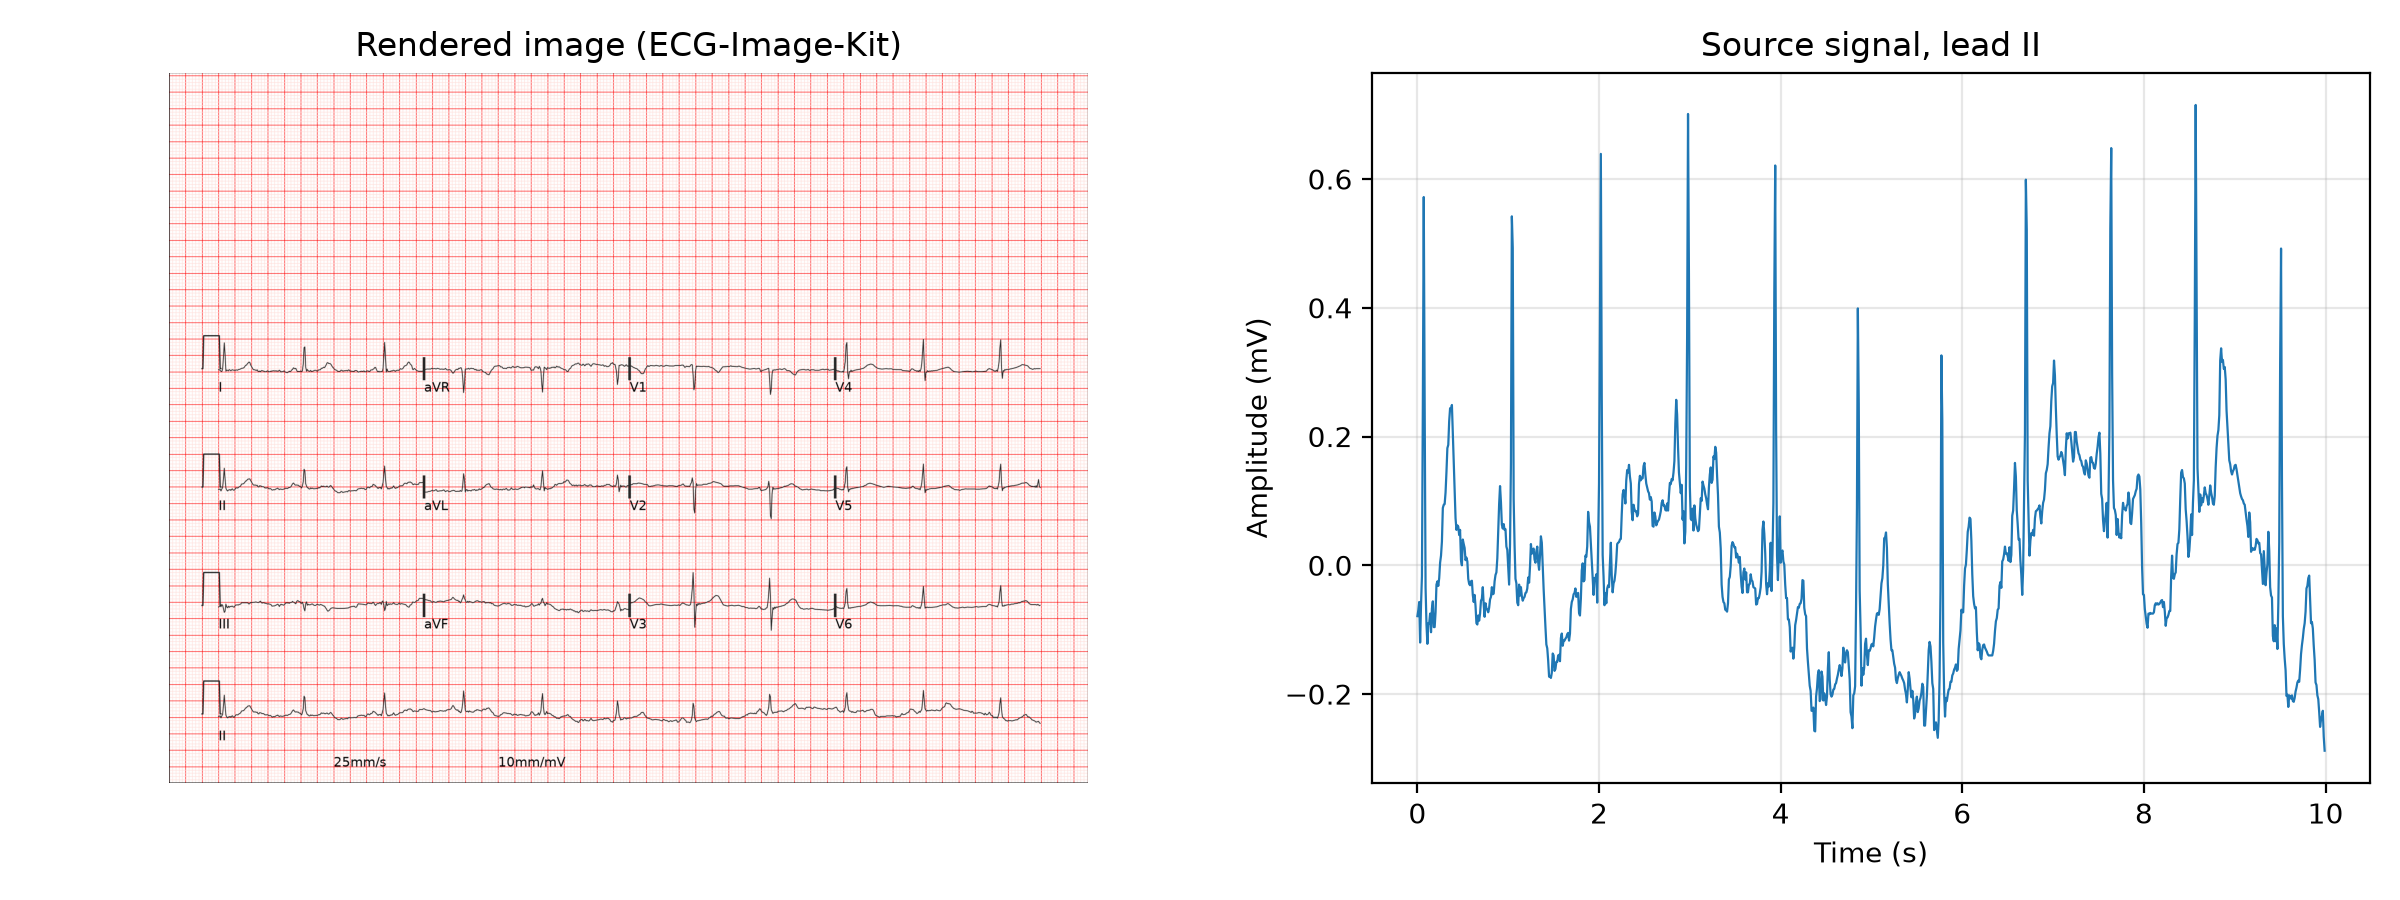
\includegraphics[width=\linewidth]{images/rendered_vs_signal.png}
  \caption{A clean rendering of PTB-XL record 00001\_lr with ECG-Image-Kit
    \cite{shivashankara_ecg-image-kit_2024} (left), and the lead II signal it was generated
    from (right). Both show 11 beats at about 0.9--1.0\,s spacing.}
  \label{fig:proto2}
\end{figure}

\textbf{Prototype 2: preprocessing and detection.}  
To test image processing for Chapter~\ref{ch:lit}, OpenCV operations were applied sequentially to a rendered ECG image (Figure~\ref{fig:proto2}). Thresholding was used to separate the ECG trace from the background, whilst also removing colour, and then used feature detection to remove the grid. A rendering of just the trace was the final result. As the final pipeline will involve all kinds of ECG images, the preprocessing will be chosen by their effectiveness.

\begin{figure}[ht]
  \centering
  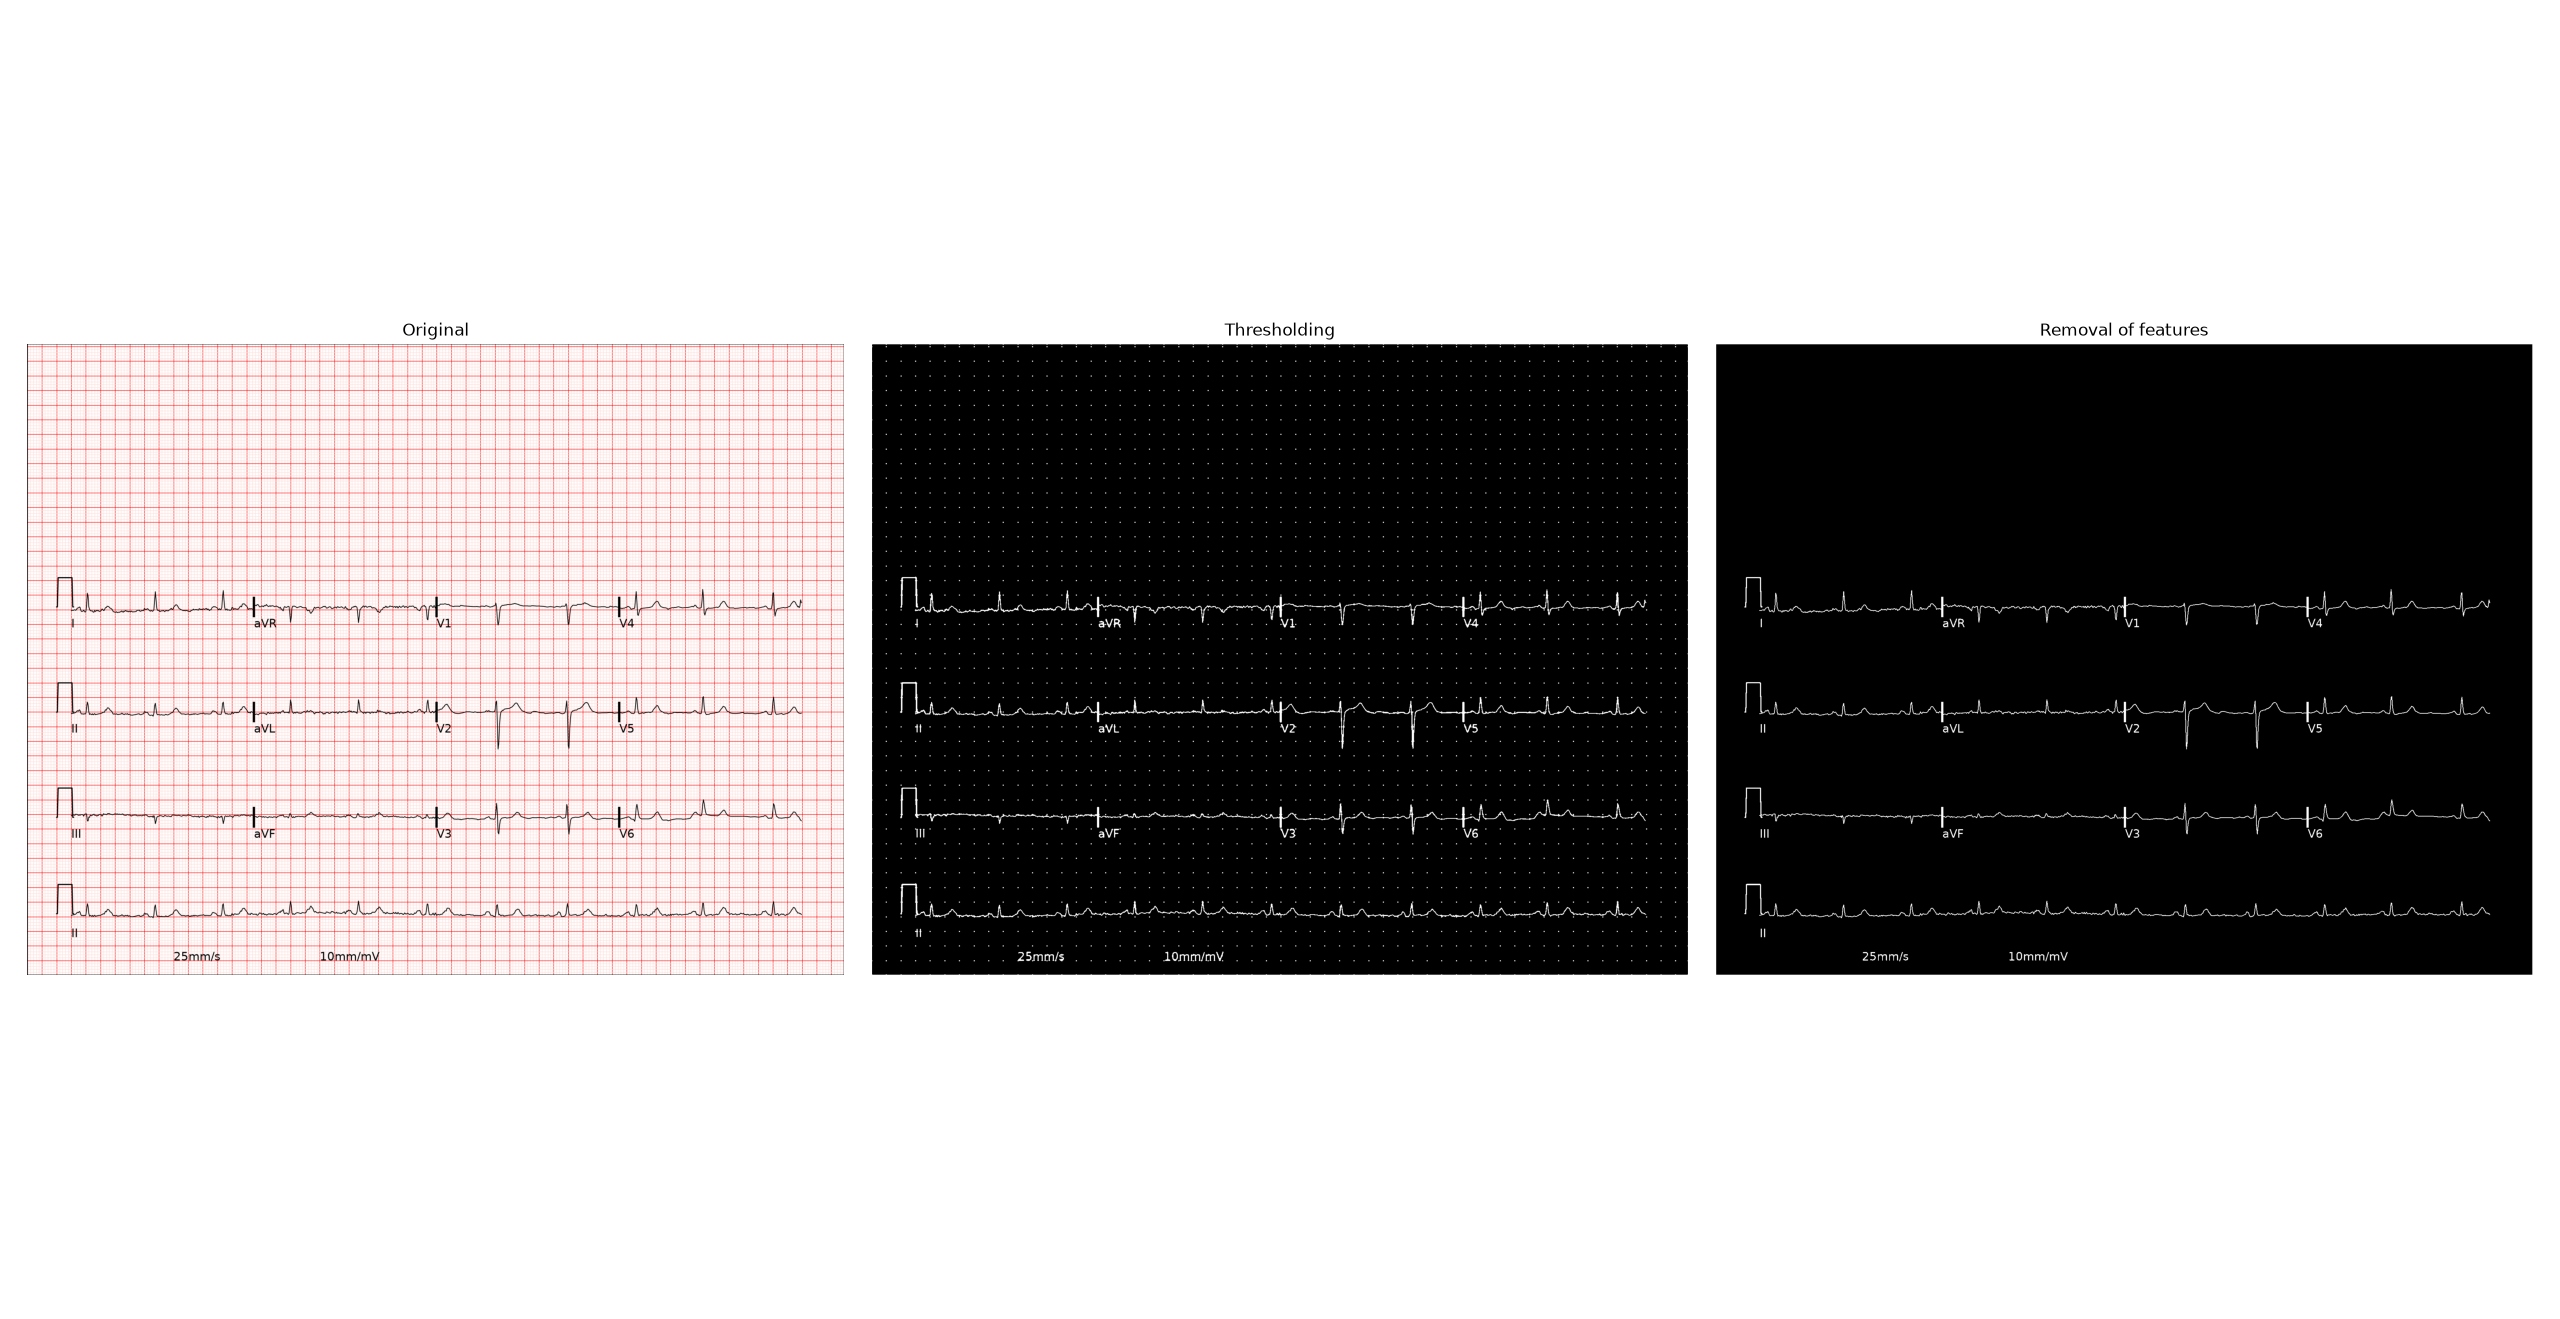
\includegraphics[width=0.9\linewidth]{images/prototype2_preprocessing.png}
  \caption{Preprocessing steps applied to a rendered ECG image.}
  \label{fig:proto2}
\end{figure}


\textbf{Prototype 3: Wireframe.}
Wireframes are drawn for the two views: the user view, which contrains the flags, the confidence scores, heatmap, and explanations. The clinical view has a short flagged list and the measured values. This protoypes demonstrates how the results will be presented to each kind of user before the interface is built, and it also the basis of our interface tested in the user study.

[TO COMPLETE]
\section{Risks}
\label{sec:feas-risks}

The full risk assessment, with the severity, likelihood and mitigation of each risk, are given in Table~\ref{tab:project-risks} and Table~\ref{tab:risks} in the Project Management section (Appendix~\ref{app:ranalysis}). The main risks for feasibility are that models trained on rendered images may not transfer to real images (R1), that trace detection may fail on poor real images (R2), rare classes may have too few cases (R3), and that there may not be enough time for the full interface (R10). Each has a fallback: the rendered-to-real gap will be reported as a result, the classifier will use the image alone if detection fails, rare classes will be reported with their counts or evaluated on rendered images only, and the interface can be reduced to uploading, flagging and the heatmap. 

% =====================================================================
\section{Summary}

The preliminary work shows that signals are able to be rendered into images to be assigned as training data. In addition, we can see the techniques used for preprocessing an image before applying it. In addition and
identifies the rendered-to-real gap and the rare classes as the main risks. The next stage is
to build the full pipeline, models, calibration, explanation and interface, and to evaluate
them as set out in Chapter~\ref{ch:method}.